%************************************************
\chapter{Multifidelity Bayesian Optimization for Accelerated Feedback Controller Tuning}\label{ch:mfbo} 
%************************************************

\section{Introduction}
\label{sec:intro}
Laboratory unit operations such as reactors and distillation columns  are often subjected to many processes in short window of time. For each new process, the control systems of these unit operations need to be re-tuned, which can be a time and labor intensive endeavor. As an example, in the distillation laboratories at BASF, operators often spend days attempting to find the best tuning parameters for a new distillation column setup, which is unacceptable given the short timelines of operating a testing laboratory. While it is possible to use model predictive control, decentralized PID controllers are often used due to their robustness and simplicity. In this work, we aim to develop a fast method tuning controllers and apply this method laboratory distillation columns.

There are a wide variety of existing tuning protocols ranging from heuristics such as Ziegler Nichols \citep{Ziegler1942} and its refinements \citep{Hang1991} to tuning using analytical equations from models via methods such as  Internal Model Control \citep{Copeland2010}. However, extending these to multi-input multi-output systems has been challenging, often requiring additional optimizations \citep{Nandong2013, Nandong2015}. Optimization-based methods have shown promise \citep{Pajares2019, Sumana2010, Rajapandiyan2012, Behroozsarand2012}, but these methods have been difficult to apply in practice due to the large number of iterations they require. Recently, Bayesian optimization, a technique for optimizing expensive to evaluate functions, has shown promise for tuning controllers \citep{NeumannBrosig2020, Fiducioso2019, Khosravi2020, Konig2020, Fujimoto2022, Brunzema2022, Khosravi2022}, but this method still often requires tens to hundreds of iterations, making it too materially expensive for laboratory chemical processes. 

In this work, we introduce a novel optimization approach that combines simulation and Bayesian optimization (BO) to effectively tune controllers. Specifically, we develop a dynamic simulation of a distillation column that is only a low fidelity approximation of the original distillation simulation. We then develop a Bayesian optimizaiton algorithm can use these simulations, despite their low fidelity, to reduce the number of iterations required to find optimal controller parameters. 

\begin{figure}
    \centering
    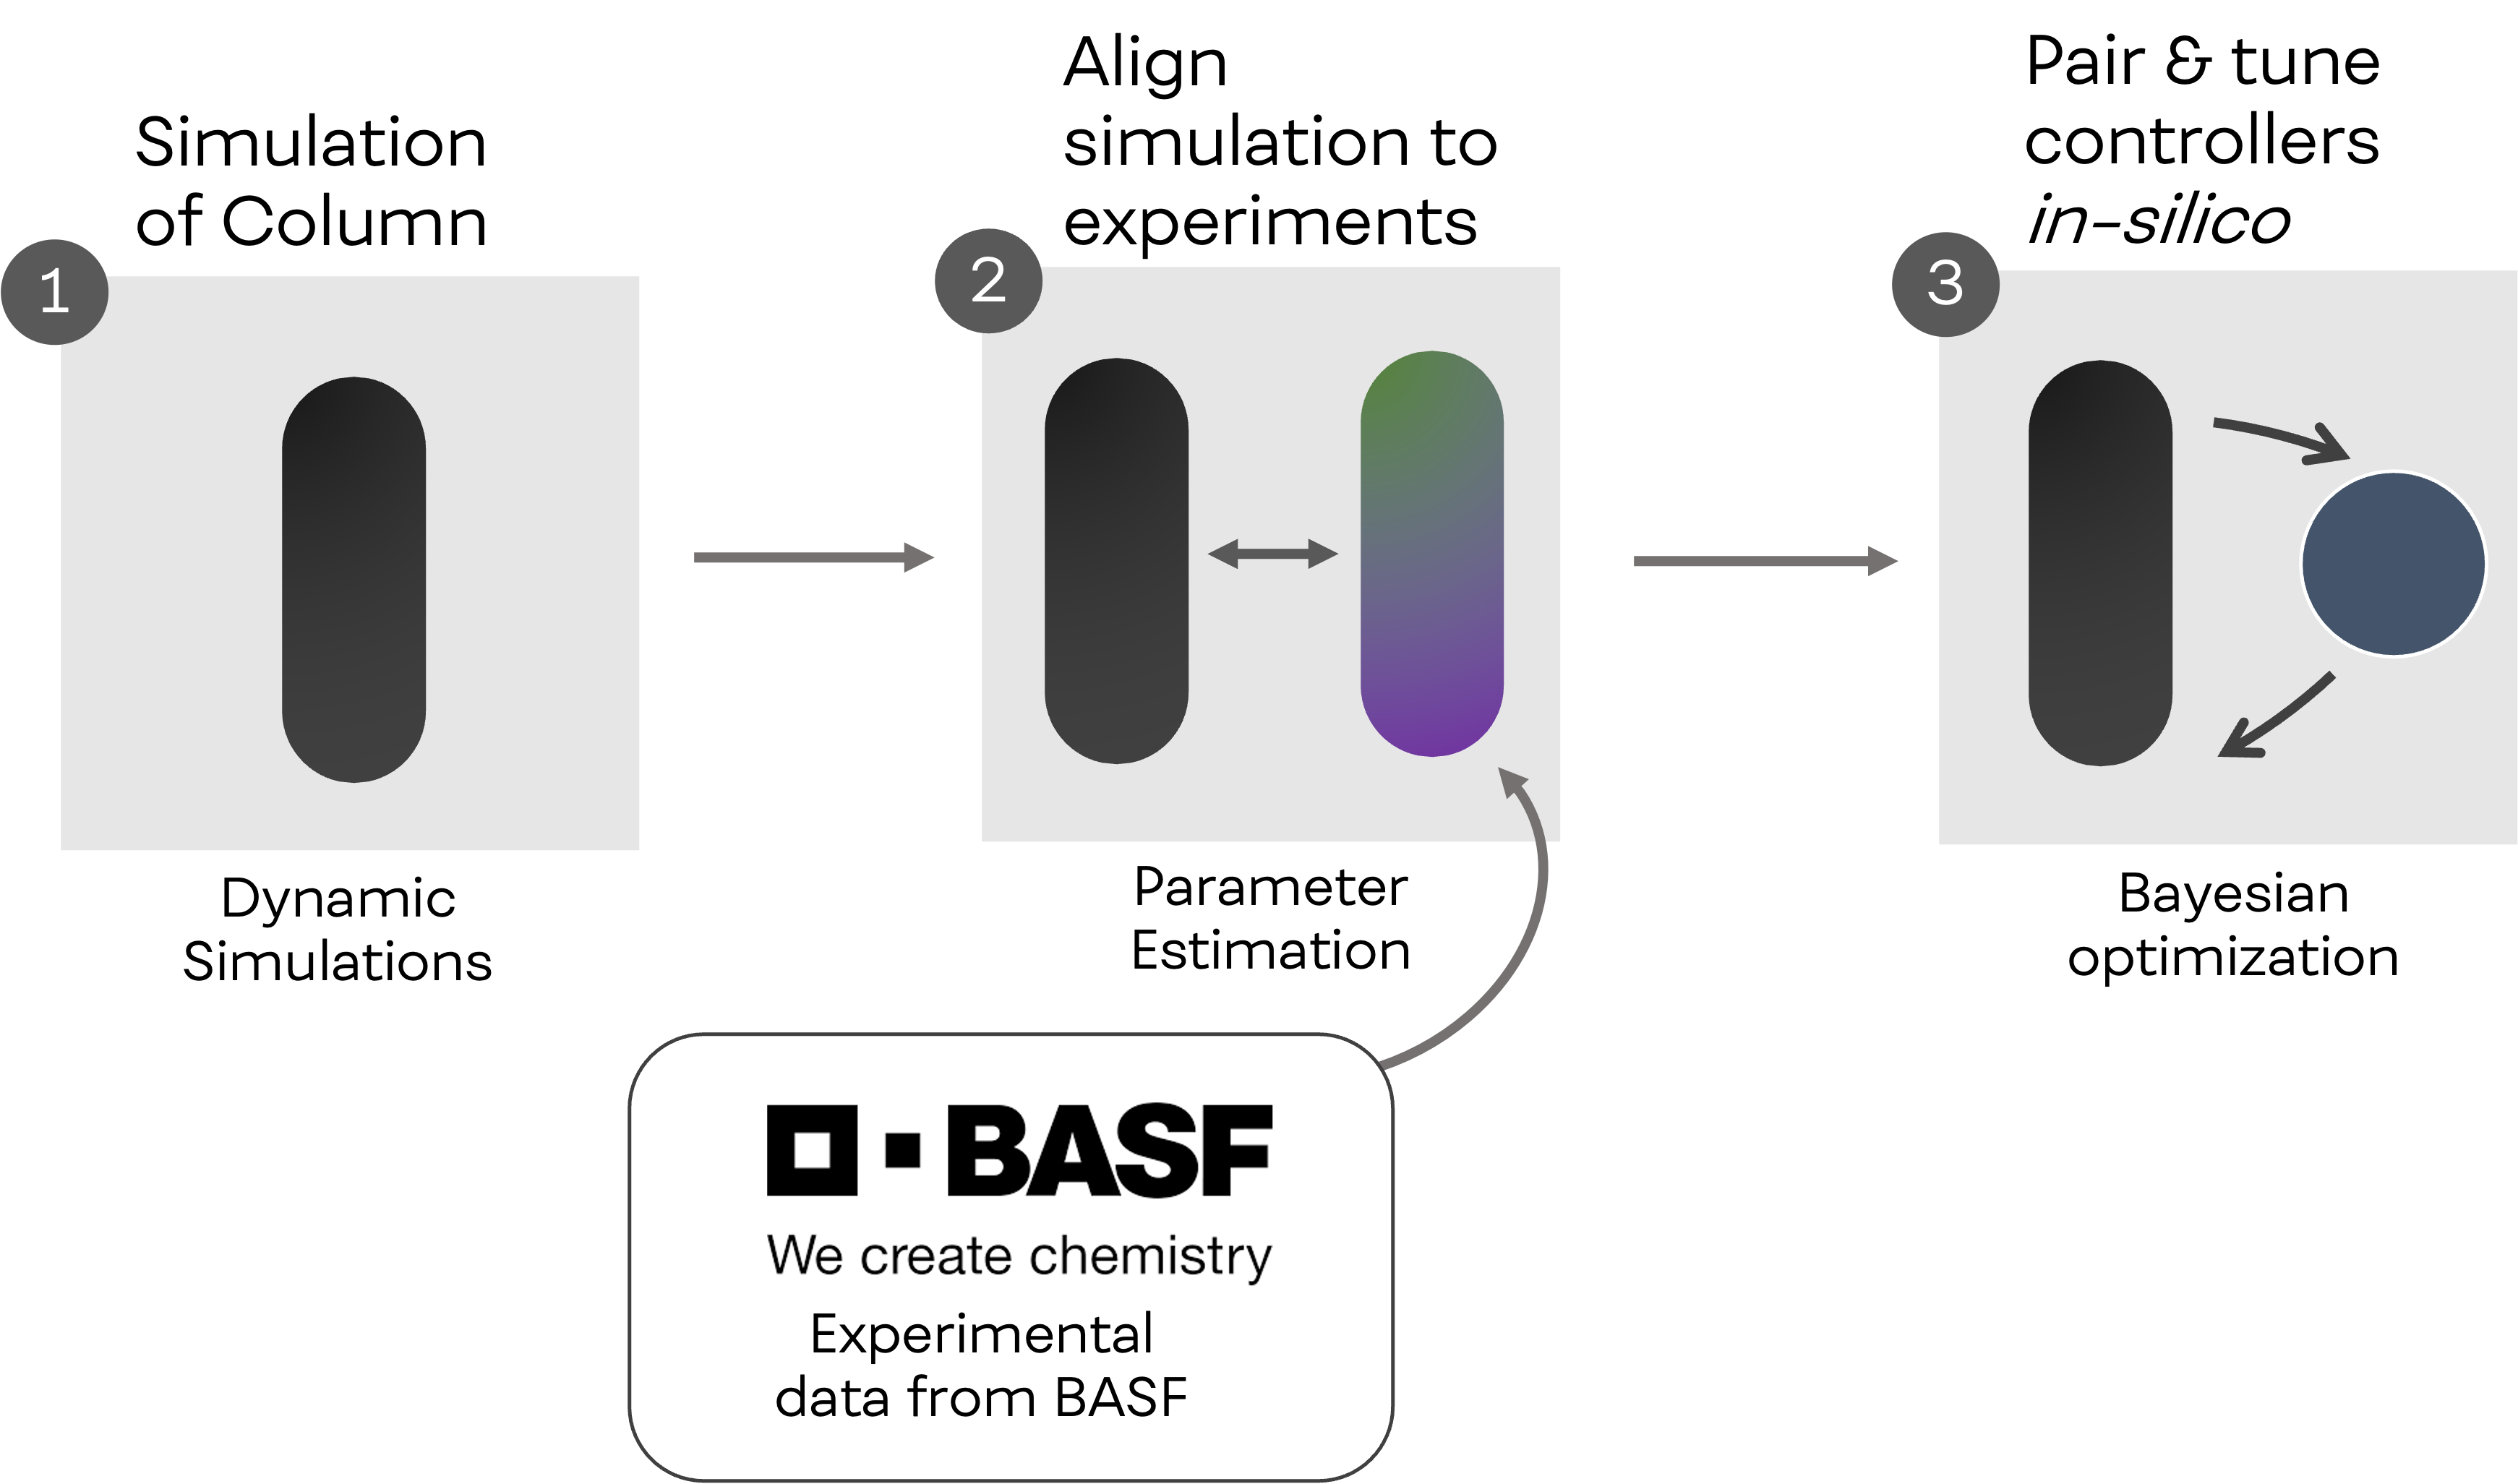
\includegraphics[width=0.8\textwidth]{figures/tuning_workflow.png}
    \caption{Three step workflow for distillation controller design and tuning. }
    \label{fig:tuning_workflow}
\end{figure}

\section{Methods}

\subsection{Controller Tuning as an Optimization Problem}

Tuning involves identifying the three parameters of the PID equation, $K^P$, $\tau_I$ and $\tau_D$:

\begin{equation}
    \label{eq:PID_defining_equation}
    u(t) = K^P e(t) + \frac{1}{\tau_I}\int_0^t e(t')dt' + \tau_D \frac{de(t)}{dt}
\end{equation}
where $u(t)$ is the controller output that is feed into the actuator (e.g., a valve) and $e(t)$ is the error at time $t$

We formulate the problem of controller design and tuning as an optimization problem. The aim is to find a set of controller pairings and tunings that will achieve desired behavior. We define good controller behavior as minimizing the integral absolute error (IAE) for each controlled variable and minimizing total controller movement (CM):
\begin{equation}
    \min_{\Omega}(IAE_1, IAE_2, IAE_3, CM_1, CM_2, CM_3)
\end{equation}

\begin{equation}
    IAE = \int_0^T \vert y_{sp}(t) - \hat y(t) \vert dt
\end{equation}

\begin{equation}
    CM = \sum_{t=1}^{T}( \vert x_t - x_{t-1} \vert)
\end{equation}
where $y_{sp}$ is the setpoint,  $\hat y$  is the value of  the variable, T is the time horizon. 

\subsection{Multi-Objective Bayesian Optimization for Controller Tuning}

We solved the controller tuning problem using multi-objective Bayesian optimization problem. Bayesian optimization is a method for rapid optimization of expensive to evaluate functions \citep{Shahriari2016}. It relies on three components: a probabilistic surrogate model of the function, an acquisition function, and an optimization algorithm.  The probabilistic surrogate model is trained on data sampled from experiments. The acquisition function determines the value of different potential experiments given the the trained probabilistic model, and the optimization algorithm is used to find the next candidate that maximizes the acquisition function.

Typically, the probabilistic model in Bayesian optimization is a Gaussian process (GP). GPs are known for having god performance in the small data regime without the need for hyperparameter tuning. These models are defined by a mean function $\mu$ and a kernel $k_{\theta}$:

\begin{equation}
    f(x)= \mathcal{GP}(\mu(x), k_{\theta}(x, x'))
\end{equation}

$\theta$ are referred to as the hyperparameters of the GP and are varied to train the GP. Given a finite set of $N$ inputs $\mathbf X = \{\mathbf x_1, \mathbf x_2, \dots, \mathbf x_N \ \vert x_i \in \mathbb R^m \}$ that correspond with outputs $\mathbf y = \{y_1, y_2, \dots y_N \vert  y_i \in \mathbb R \}$, the GP is a multivariate Gaussian distribution:

\begin{equation}
    f(\mathbf X) \sim \mathcal N(\mu_{\theta}(\mathbf X), k_{\theta}(\mathbf X, \mathbf X'))
\end{equation}

In this work, we used the Matérn 5/2 kernel and set the mean function to zero, as full expressive capability comes can come from the kernel. To train the GP, we minimized the negative log likelihood:

\begin{equation}
    \log p(y \vert X, \theta) = -\underbrace{\frac{1}{2}(y-\tilde \mu_{\theta}(\mathbf X))^T k_{\theta}(\mathbf X, \mathbf X)^{-1}(y- \tilde\mu_{\theta}(\mathbf X)) }_{\text{Data  fit}}- \underbrace{\frac{1}{2} \log{\vert \tilde k_{\theta}(\mathbf X, \mathbf X) \vert} - \frac{d}{2}\log{2 \pi}}_{\text{Complexity penalty}}
\end{equation}

We trained an independent GP to predict each controller objective (IAE, CM) given the relevant controller parameters.  

Since our problem is multi-objective, we used a multi-objective acquisition function, namely the q Noisy Expected Hypervolume Improvement (qNEHVI). This acquisition function has a balance of computational efficiency and fidelity resulting in an ability to find the pareto front of trade-offs between objectives quickly. 

\subsection{Leveraging Simulations via Multifidelity Bayesian Optimization}

We desired to see if simulations could accelerate controller tuning. We developed a differential equation simulation of a distillation column that was is aligned to experimental data using both steady state and dynamic parameter estimation (see Supplementary Material for full details). To leverage the simulation, we used a multi-task GP that could be trained on both the less abundant high fidelity experimental data and the more abundant low fidelity simulation data. We hoped that the multi-task GP could learn the correlation between the simulation and the experimental data and thus make better predictions on the experiments with less data.

In practice, we optimized the high fidelity task when selecting  a new set of controller parameters ton run an experiment in the laboratory. Then, while waiting for the laboratory results, we used optimize the lower fidelity task using the differential equation simulation with the most recently estimated parameters. 

\subsection{Case Study}

In order to base our simulations in reality, we collected experimental data for separation of a 50/50 methanol-water mixture at the laboratories of BASF SE in a 80 tray column with one bubble cap on each stage. The column was kept at approximately 800 mbar vacuum, and a Julabo evaporator was used as the reobiler. The column occupies approximately three stories in the BASF lab.  Three days of data were collected, one of which is used for parameter estimation and the rest for validation. A simulation of this column after parameter estimation to the experimental data was used as the "experiment" in the BO studies.

\section{Results}

\section{Conclusion}